% Partie : set-theory
% Chapitre : ordinals
% Section : idea

\documentclass[../../../include/open-logic-section]{subfiles}

\begin{document}

\olfileid[fr]{sth}{ordinals}{idea}

\olsection{L'idée générale d'un ordinal}

Considérons les nombres naturels dans leur ordre habituel :
\begin{center}
	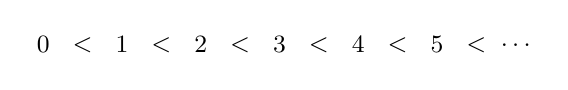
\begin{tikzpicture}
	\foreach \x/\xtext in {0, 1, 2, 3, 4, 5}
	{
		\node (\x a) at (\x, 1) {\small{$\x$}};
		\node (\x a) at (\x.5, 1) {\small{$<$}};
	}
	\node (ldots) at (6, 1) {\small{$\ldots$}};
	\end{tikzpicture}
\end{center}
Nous appelons cela, dans le jargon, une suite de type $\omega$.
Cet ordre général se retrouve dans notre construction initiale des
étapes de la hiérarchie des ensembles. Supposons maintenant que nous
déplacions $0$ à la fin de cette suite, de sorte qu'il vienne après
tous les autres nombres :
\begin{center}
	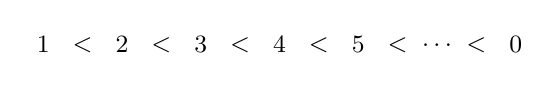
\begin{tikzpicture}
	\foreach \x/\xtext in {1, 2, 3, 4, 5}
	{
		\node (\x a) at (\x, 1) {\small{$\x$}};
		\node (\x a) at (\x.5, 1) {\small{$<$}};
	}
	\node (ldots) at (6, 1) {\small{$\ldots$}};
	\node (bea) at (6.5, 1) {\small{$<$}};
	\node (noa) at (7, 1) {\small{$0$}};
	\end{tikzpicture}
\end{center}
Les éléments sont les mêmes, mais leur ordre a fondamentalement changé :
le premier n'avait pas de dernier élément, tandis que le nouvel ordre
en a un. Celui-ci se compose en effet d'une suite de type $\omega$
d'éléments ($1, 2, 3, 4, 5, \ldots$), suivie d'un élément
supplémentaire. C'est une suite de type $\omega+1$.

Nous pouvons obtenir, avec ces seuls éléments, encore d'autres types
d'ordre. Considérons par exemple tous les nombres pairs (dans leur
ordre naturel), suivis de tous les nombres impairs (dans leur ordre
naturel) :
\begin{center}
	\begin{tikzpicture}
	\node(a1) at (1,1) {\small{$0$}};
	\node(a2) at (1.5,1) {\small{$<$}};
	\node(a3) at (2,1) {\small{$2$}};
	\node(a4) at (2.5,1) {\small{$<$}};
	\node(a5) at (3,1) {\small{$4$}};
	\node(a6) at (3.5,1) {\small{$<$}};
	\node(dots) at (4,1) {\small{$\ldots$}};
	\node(aaoe) at (4.5,1) {\small{$<$}};
	\node(b1) at (5,1) {\small{$1$}};
	\node(b2) at (5.5,1) {\small{$<$}};
	\node(b3) at (6,1) {\small{$3$}};
	\node(b4) at (6.5,1) {\small{$<$}};
	\node(b5) at (7,1) {\small{$\ldots$}};
	\end{tikzpicture}
\end{center}
Il s'agit d'une suite de type $\omega$ suivie d'une autre suite de
type $\omega$ : une suite de type $\omega+\omega$.

Nous pourrions poursuivre. Mais ce que nous voulons, c'est une manière
générale de comprendre ces différents \emph{ordres}.

\end{document}
